%%%%%%%%%%%%%%%%%%%%%%%%%%%%%%%%%%%%%%%%%
% Beamer Presentation
% LaTeX Template
% Version 1.0 (10/11/12)
%
% This template has been downloaded from:
% http://www.LaTeXTemplates.com
%
% License:
% CC BY-NC-SA 3.0 (http://creativecommons.org/licenses/by-nc-sa/3.0/)
%
%%%%%%%%%%%%%%%%%%%%%%%%%%%%%%%%%%%%%%%%%

%----------------------------------------------------------------------------------------
%	PACKAGES AND THEMES
%----------------------------------------------------------------------------------------

\documentclass{beamer}

\mode<presentation> {

% The Beamer class comes with a number of default slide themes
% which change the colors and layouts of slides. Below this is a list
% of all the themes, uncomment each in turn to see what they look like.

%\usetheme{default}
%\usetheme{AnnArbor}
%\usetheme{Antibes}
%\usetheme{Bergen}
%\usetheme{Berkeley} % Neat Contents on left
%\usetheme{Berlin}
%\usetheme{Boadilla}
%\usetheme{CambridgeUS} % Neat but breadcrumbs at top
%\usetheme{Copenhagen}
%\usetheme{Darmstadt}
%\usetheme{Dresden}
%\usetheme{Frankfurt}
%\usetheme{Goettingen} %Neat contents on right
\usetheme{Hannover} %Neat contents on left
%\usetheme{Ilmenau}
%\usetheme{JuanLesPins}
%\usetheme{Luebeck}
%\usetheme{Madrid}
%\usetheme{Malmoe}
%\usetheme{Marburg} % Contents on right in contrast color
%\usetheme{Montpellier}
%\usetheme{PaloAlto} % Contents on left
%\usetheme{Pittsburgh}
%\usetheme{Rochester}
%\usetheme{Singapore}
%\usetheme{Szeged}
%\usetheme{Warsaw}

% As well as themes, the Beamer class has a number of color themes
% for any slide theme. Uncomment each of these in turn to see how it
% changes the colors of your current slide theme.

%\usecolortheme{albatross}
%\usecolortheme{beaver}
%\usecolortheme{beetle}
%\usecolortheme{crane}
%\usecolortheme{dolphin}
%\usecolortheme{dove}
%\usecolortheme{fly}
%\usecolortheme{lily}
%\usecolortheme{orchid}
%\usecolortheme{rose}
%\usecolortheme{seagull}
\usecolortheme{seahorse}
%\usecolortheme{whale}
%\usecolortheme{wolverine}

%\setbeamertemplate{footline} % To remove the footer line in all slides uncomment this line
%\setbeamertemplate{footline}[page number] % To replace the footer line in all slides with a simple slide count uncomment this line

%\setbeamertemplate{navigation symbols}{} % To remove the navigation symbols from the bottom of all slides uncomment this line
}

\usepackage{graphicx} % Allows including images
\usepackage{booktabs} % Allows the use of \toprule, \midrule and \bottomrule in tables

%----------------------------------------------------------------------------------------
%	TITLE PAGE
%----------------------------------------------------------------------------------------

\title[Improving Outcomes in Pancreatic Surgery]{An investigation of the clinical utility of preoperative cardiopulmonary exercise testing in patients undergoing major pancreatic surgery.} % The short title appears at the bottom of every slide, the full title is only on the title page

\author{Vishnu V Chandrabalan} % Your name
\institute[UoG] % Your institution as it will appear on the bottom of every slide, may be shorthand to save space
{
University of Glasgow \\ % Your institution for the title page
\medskip
% \textit{john@smith.com} % Your email address
}
\date{\today} % Date, can be changed to a custom date

\begin{document}

\begin{frame}
\titlepage % Print the title page as the first slide
\end{frame}

\begin{frame}
\frametitle{Overview} % Table of contents slide, comment this block out to remove it
\tableofcontents % Throughout your presentation, if you choose to use \section{} and \subsection{} commands, these will automatically be printed on this slide as an overview of your presentation
\end{frame}

%----------------------------------------------------------------------------------------
%	PRESENTATION SLIDES
%----------------------------------------------------------------------------------------

%------------------------------------------------
\section{Introduction}
\subsection{Pancreatic cancer}
\begin{frame}
	\frametitle{Pancreatic cancer} %Epidemiology/outcomes
	\begin{block}{The Problem}
		\begin{itemize}
			\item 10th common but 5th common cause of cancer death
			\item Survival	1-yr: 20.8\%, 5-yr: 3.3\%, 10yr: 1.1\%
			\item Operable disease : approx 15\%
		\end{itemize}
	\end{block}
	\begin{block}{Treatment}
		\begin{itemize}
			\item Surgery + adjuvant chemotherapy only chance of cure
		\end{itemize}
	\end{block}
	\begin{block}{Pancreaticoduodenectomy}
		\begin{itemize}
			\item Complex surgery with 50\% morbidity
			\item Performed only in specialist centres
			\item Patient fitness is as important as tumour factors
		\end{itemize}
	\end{block}
\end{frame}

\begin{frame}
	\frametitle{Pancreaticoduodenectomy}
	\begin{columns}[t]
		\column{0.45\textwidth}
		\begin{figure}
			\centering
			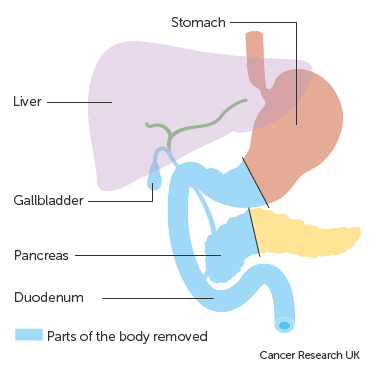
\includegraphics[width=0.8\linewidth]{whipple_schematic_pre}
			\label{fig:whipple_schematic_pre}
		\end{figure}
		{\scriptsize
			\textbf{Structures removed:}
			\begin{itemize}
			\item Head of pancreas
			\item Distal stomach, duodenum, proximal jejunum
			\item  Common bile duct, gallbladder
			\item Lymphadenectomy
			\item Venous resection in some
		\end{itemize}}
	
		
		\column{0.45\textwidth}
		\begin{figure}
			\centering
			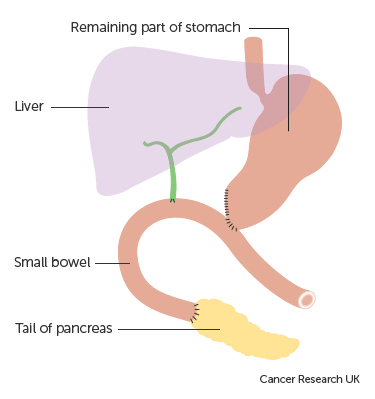
\includegraphics[width=0.8\linewidth]{whipple_schematic_post}
			\label{fig:whipple_schematic_post}
		\end{figure}
		{\scriptsize
		\textbf{Reconstruction:}
		\begin{itemize}
			\item Pancreaticojejunostomy (25\% leak rate)
			\item Hepaticojejunostomy
			\item Gastrojejunostomy
		\end{itemize}
		}
	\end{columns}
\end{frame}

\begin{frame}
	\frametitle{Patient selection}
	 
	
\end{frame}

\subsection{CPET}

\begin{frame}
	\frametitle{Respiratory compensation of lactic acidosis} 
	\begin{figure}
		\centering
		\includegraphics[width=0.7\linewidth]{CellRespiration}
		\label{fig:CellRespiration}
	\end{figure}
	\centering
	$H^+ + HCO3^- \Longleftrightarrow H_2CO_3 \Longleftrightarrow H_2O + CO_2$
		
	

\end{frame}

\begin{frame}
	\frametitle{Determination of Anaerobic Threshold}
	\begin{figure}[htbp]
		\centering
		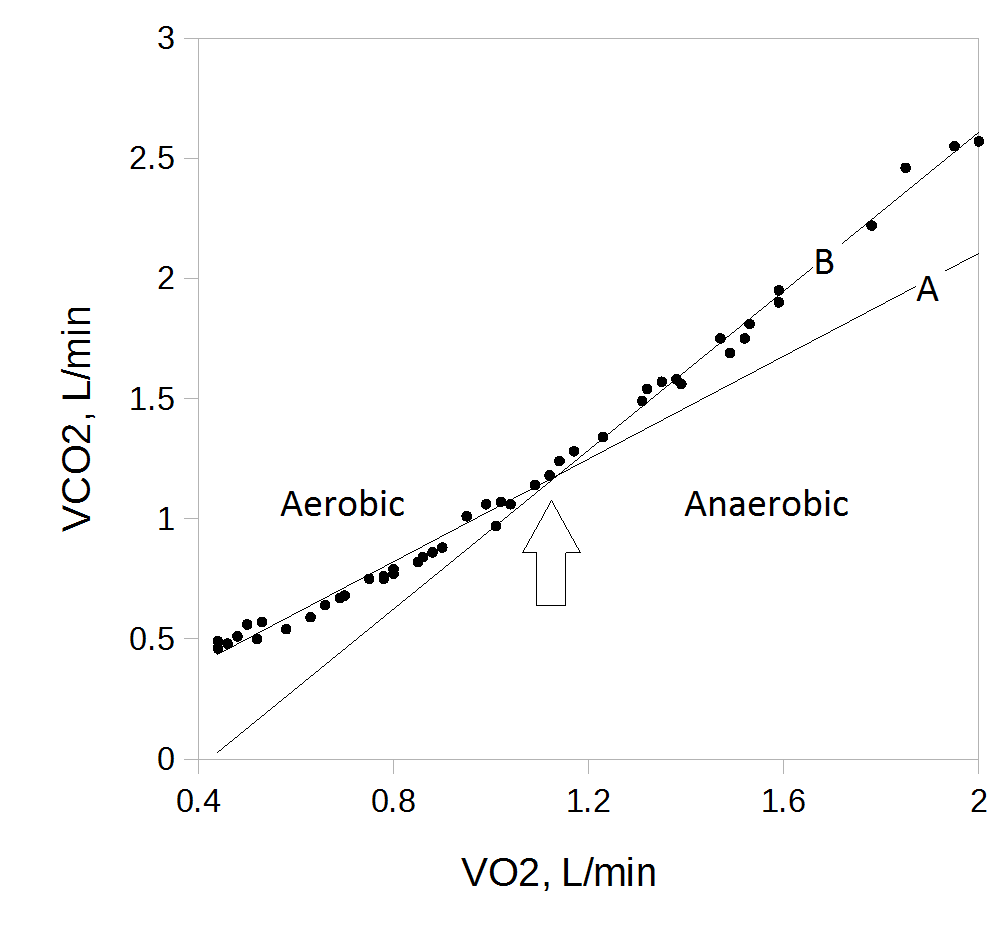
\includegraphics[width=0.7\linewidth]{../Figures/cpet_vslope}
		%\caption{Determination of $\dot{V}_{O_2}$AT by the V-slope method.}
		\label{fig:cpet_vslope}
	\end{figure}
\end{frame}

\begin{frame}
	\frametitle{Role of CPET in preoperative assessment}
	\begin{itemize}
		\item General Surgery
		\item Oesophago-gastric surgery
		\item Bariatric surgery
		\item Liver transplantation
		\item Thoracic surgery
		\medskip
		\item Little evidence in pancreatic surgery in 2010
		
	\end{itemize}
\end{frame}

\begin{frame}
	\frametitle{Aims of Thesis}
	\begin{enumerate}
		\item To evaluate the clinical utility of preoperative CPET in predicting postoperative adverse events after pancreaticoduodenectomy.
		\item To examine the patient factors that are related to cardiopulmonary exercise physiology with particular attention to the effect of obstructive jaundice and body composition.
		\item To examine the effect of preoperative systemic inflammation and poor aerobic capacity on the magnitude of the post-operative systemic inflammatory response.
		\item To examine the value of serial daily postoperative markers of systemic inflammatory response in the prediction of post-operative complications.
	\end{enumerate}
\end{frame}

\section{Methods}
\begin{frame}
	\frametitle{Patients and Methods}
	\begin{enumerate}
		\item Patients undergoing pancreaticoduodenectomy at Glasgow Royal Infirmary
		\item August 2008 - August 2012
		\item Prospectively maintained MS Access database
		\item Preoperative data - Bloods, co-morbidity including POSSUM Physiology Score, stent information
		\item Cardiopulmonary exercise testing
		\item Prospective recording of complications using ISGPS or Clavie-Dindo classification
		\item Serial measurements of biochemical parameters during first postoperative week
	\end{enumerate}
\end{frame}

% Discuss the results in the context of a patient.
% 63 yr old female with BMI of 35 presents with painless OJ
% PMH - HTN, T2DM, smoked 10/day for 40 yrs
% Bloods: Bil 180, CRP 22, Alb 30
% Investigations reveal an operable tumour of the head of the pancreas
% How would this patient have been managed 10 years ago?
\section{Case study}
\begin{frame}
	\frametitle{A typical patient}
	\begin{itemize}
		\item 63 yr old female with BMI of 35 presents with painless OJ
		\item PMH - HTN, T2DM, smoked 10/day for 40 yrs
		\item Bloods: Bil 180, CRP 22, Alb 30
		\item Imaging: Resectable tumour of head of pancreas
		\item How would this patient have been managed 10 years ago?
	\end{itemize}
\end{frame}

\begin{frame}
	\frametitle{10 years ago...}
	\begin{itemize}
		\item Non-dynamic measures of fitness - ECG, PFTs, ASA, ECHO
		\item Routine biliary drainage
		\item No objective methods to predict complications other than pancreatic leak
		\item Impact of postoperative SIRS on complications - no clinical utility
		\item Limited ability to identifying patients at risk of complications
		\item ERAS principles not universally applied
		\item No prehabilitation
	\end{itemize}
\end{frame}

\begin{frame}
	\frametitle{Now... }
	\begin{itemize}
		\item CPET in all or selected cases (evidence from other patient groups)
		\item Routine biliary drainage no longer indicated
		\item Enhanced recovery more widespread
		\medskip
		\hrule
		\medskip
		\item Reluctance to perform CPET in jaundiced patients
		\item No recognised thresholds for CPET parameters
		\item No clear thresholds for post-op inflammatory markers in predicting complications
		\item Poor understanding of impact of obesity on preop function and postop outcomes
		\item No prehabilitation
	\end{itemize}
\end{frame}

\section{Results}
\subsection{CPET vs Outcomes}
\begin{frame}
	\frametitle{CPET and Postoperative Outcomes}
	\begin{block}{\textbf{Complications}}
		Low $\dot{V}_{O_2}$AT associated with pancreatic fistula (16\% vs 35\%) \\
		Not associated with cardio-respiratory complications or mortality
	\end{block}
	
	\begin{block}{\textbf{Length of stay}}
		Low $\dot{V}_{O_2}$AT associated with longer hospital stay (14 vs 20 days)\\
		Not associated with critical care stay or admissions
	\end{block}
	
	\begin{block}{\textbf{Adjuvant Therapy}}
		Low $\dot{V}_{O_2}$AT associated with non-progression to adjuvant therapy after surgery.
	\end{block}
	
\end{frame}


\subsection{CPET vs Jaundice}
\begin{frame}
	\frametitle{CPET and Jaundice}
	\begin{columns}[t]
		\column{0.5\textwidth}
			\begin{figure}
				\centering
				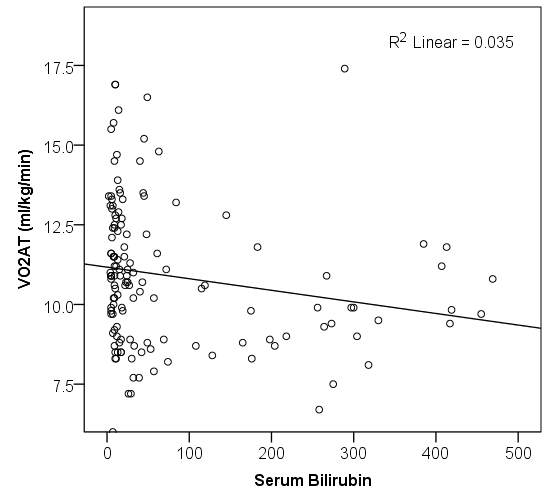
\includegraphics[width=\textwidth]{../Figures/cpet_oj_scatter_at_bil}
				\caption{$\dot{V}_{O_2}$AT versus serum bilirubin}
				\label{fig:cpet_oj_scatter_at_bil}
			\end{figure}
			
		\column{0.5\textwidth}
			\begin{figure}
				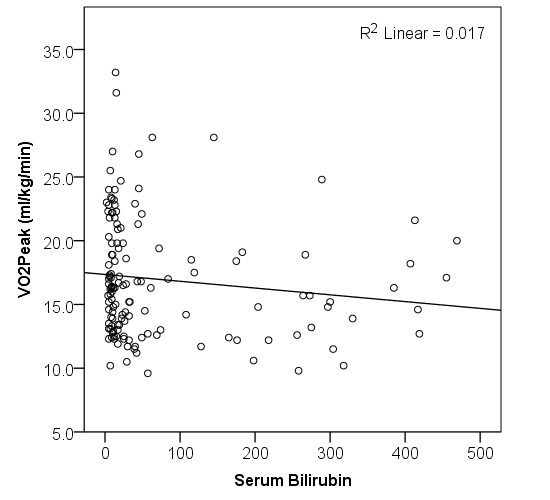
\includegraphics[width=\textwidth]{../Figures/cpet_oj_scatter_peak_bil}
				\caption{$\dot{V}_{O_2}$Peak versus serum bilirubin}
				\label{fig:cpet_oj_scatter_peak_bil}
			\end{figure}
	\end{columns}
	
\end{frame}

\subsection{CPET vs Body Composition}
\begin{frame}
	\frametitle{CPET and Body Composition}
\end{frame}

\subsection{Systemic inflammation}

\begin{frame}
	\frametitle{Preop Pathophysiology and Postoperative Systemic Inflammation}
	\begin{block}{title}
		Preoperative inflammatory status of the patient and obstructive jaundice play an important role in modulating postoperative systemic inflammation which may not simply be due to the effect of surgery and its sequelae.
	\end{block}
\end{frame}

\begin{frame}
	\frametitle{Postoperative Systemic Inflammation and Outcomes}
\end{frame}




\begin{frame}
\frametitle{Multiple Columns}
\begin{columns}[c] % The "c" option specifies centered vertical alignment while the "t" option is used for top vertical alignment

\column{.45\textwidth} % Left column and width
\textbf{Heading}
\begin{enumerate}
\item Statement
\item Explanation
\item Example
\end{enumerate}

\column{.5\textwidth} % Right column and width
Lorem ipsum dolor sit amet, consectetur adipiscing elit. Integer lectus nisl, ultricies in feugiat rutrum, porttitor sit amet augue. Aliquam ut tortor mauris. Sed volutpat ante purus, quis accumsan dolor.

\end{columns}
\end{frame}

\begin{frame}
\frametitle{Table}
\begin{table}
\begin{tabular}{l l l}
\toprule
\textbf{Treatments} & \textbf{Response 1} & \textbf{Response 2}\\
\midrule
Treatment 1 & 0.0003262 & 0.562 \\
Treatment 2 & 0.0015681 & 0.910 \\
Treatment 3 & 0.0009271 & 0.296 \\
\bottomrule
\end{tabular}
\caption{Table caption}
\end{table}
\end{frame}

%------------------------------------------------





%------------------------------------------------

\begin{frame}[fragile] % Need to use the fragile option when verbatim is used in the slide
\frametitle{Verbatim}
\begin{example}[Theorem Slide Code]
\begin{verbatim}
\begin{frame}
\frametitle{Theorem}
\begin{theorem}[Mass--energy equivalence]
$E = mc^2$
\end{theorem}
\end{frame}\end{verbatim}
\end{example}
\end{frame}

%------------------------------------------------

\begin{frame}
\frametitle{Figure}
Uncomment the code on this slide to include your own image from the same directory as the template .TeX file.
%\begin{figure}
%\includegraphics[width=0.8\linewidth]{test}
%\end{figure}
\end{frame}

%------------------------------------------------

\begin{frame}[fragile] % Need to use the fragile option when verbatim is used in the slide
\frametitle{Citation}
An example of the \verb|\cite| command to cite within the presentation:\\~

This statement requires citation \cite{p1}.
\end{frame}

%------------------------------------------------

\begin{frame}
\frametitle{References}
\footnotesize{
\begin{thebibliography}{99} % Beamer does not support BibTeX so references must be inserted manually as below
\bibitem[Smith, 2012]{p1} John Smith (2012)
\newblock Title of the publication
\newblock \emph{Journal Name} 12(3), 45 -- 678.
\end{thebibliography}
}
\end{frame}

%------------------------------------------------

\begin{frame}
\Huge{\centerline{The End}}
\end{frame}

%----------------------------------------------------------------------------------------

\end{document} 